\section{Grundlagen}\label{sec:grundlagen}
\textit{Closed Innovation} ist eine Variante den Wissensaustausch
zur Entwicklung einer \textit{Innovation}
innerhalb eines \textit{Innovationsprozesses} zu organisieren.

In der Litaratur finden sich für die beiden letzeren Begriffe verschiedene Beschreibungen.
Im folgenden werden die in dieser Arbeit verwendeten Definitionen vorgestellt.

\subsection{Innovation}\label{sec:grundlagen-inno}
Bevor die Begriffe \textit{Closed} und \textit{Open Innovation} näher betrachtet werden,
ist es notwendig den Begriff \textit{Innovation} an sich zu definieren.
Verschiedene Autoren definieren diesen Begriff auf unterschiedliche Arten.
In \cite[5]{hauschildt2016innovationsmanagement} ist eine Auswahl verschiedener Definitionen dargestellt.
Diese werden zusammengefasst zu der allgemeinen Aussage:
\begin{quote}
    \enquote{Innovationen sind qualitativ neuartige Produkte oder Verfahren,
    die sich gegenüber einem Vergleichszustand \enquote{merklich} [...] unterscheiden}
    \cite[4]{hauschildt2016innovationsmanagement}
\end{quote}

In \cite[9]{herzog2011} wird ein solches neuartiges Produkt oder Verfahen als \textit{Invention} bezeichnet und erst durch kommerzielle Verwertung zur \textit{Innovation}.
Die vorliegende Arbeit folgt dieser Definition.
Es gilt somit:
\begin{equation*}
    Innovation = Invention + kommerzielle~Verwertung
\end{equation*}

Hierbei ist zu beachten, dass der Begriff sich nicht nur auf Produkte bezieht, welche vermarktet werden,
sonder auch auf Prozesse, welche innerhalb der Produktion genutzt werden.

\subsection{Innovationsprozess}\label{sec:grundlagen-prozess}
Um Ideen und Innovationen zu entwickeln und zu vermarkten durchlaufen diese zunächst einen Innovationsprozess.
Nach \cite[10\psq]{herzog2011} besteht dieser Prozess aus drei Phasen:
\begin{enumerate}
    \item Im \textit{Frontend of Innovation} werden neue Ideen geschaffen, ausgewählt, sowie auf technologische Machbarkeit und mögliche Marktakzeptanz hin bewertet.
    \item Anschließend werden ausgewählte Ideen realisiert und entwickelt.
    \item Zuletzt wird die Vermarktung der Entwicklungsergebnisse geplant und durchgeführt.
\end{enumerate}

\subsection{Closed Innovation}\label{sec:grundlagen-closed}

\paragraph{Ursprung}
Das \textit{Closed Innovation}-Modell ist das vorherschende Innovationsmodell im 20. Jahrhundert.
Es spiegelt die damals vorherschende Wissensumgebung wider.
Unter Wissenschaftlern ist es verpönt ihre Fähigkeiten zu Nutzen um wirtschaftliche Probleme zu lösen.

Um dennoch Innovationen anzutreiben und so den kommerziellen Erfolg zu sichern,
sind Unternhemen gezwungen selbst in \ac{fe} zu investieren.
Da in anderen Unternehmen das notwendige Wissen nicht aufgebaut ist,
müssen Unternehmen innerhalb ihrer \ac{fe}-Organisation das gesamte Spektrum von den Grundlagen bis hin zum fertigen Produkt abdecken.
Voraussetzung hierfür ist die Akquise von talentierten Mitarbeitern.

\todo[inline]{Geschichte etwas ausführlicher}

\paragraph{Prinzipien}
Implizit ergeben sich so die Prinzipien der \textit{Closed Innovation} (nach \cite[19]{herzog2011}):
\begin{itemize}
    \item Ein Unternehmen sollte die talentiertesten Mitarbeiter anstellen.
    \item Um von Innovationen zu profitieren, müssen diese innerhalb des Unternehmens den gesamten Innovationsprozess durchlaufen (Vom Entdecken, über das Entwicklen bis hin zur Vermarktung)
    \item Um ein Produkt als erstes auf den Markt zu bringen, muss eine Entdeckung innerhalb des eingenen Unternehmens entstehen.
    \item Durch die Markteinführung als erstes Unternehmen gewinnt es den Wettbewerb
    \item Investiert ein Unternehmen am meisten in \ac{fe}, so entstehen dort die besten Ideen, was wiederum den Wettbewerb gewinnt.
    \item Damit andere Unternehmen nicht von den eigenen Entdeckungen profitieren, gilt es das geistige Eigentum zu schützen.
\end{itemize}

\paragraph{Modell}
Aus diesen Regeln folgt das in \autoref{fig:closedInnovation} dargestellte Modell.
Der gesamte Innovatoinsprozess spielt sich innerhalb der Grenzen des Unternehmes ab.
Eine Innovation beginnt immer durch eine Idee innerhalb des Unternehmens,
wird durch die firmeneigene \ac{fe}-Abteilung entwickelt
und schließlich auf dem bestehenden Markt des Unternehmens kommerzialisiert.

\begin{figure}[ht!]
    \centering
    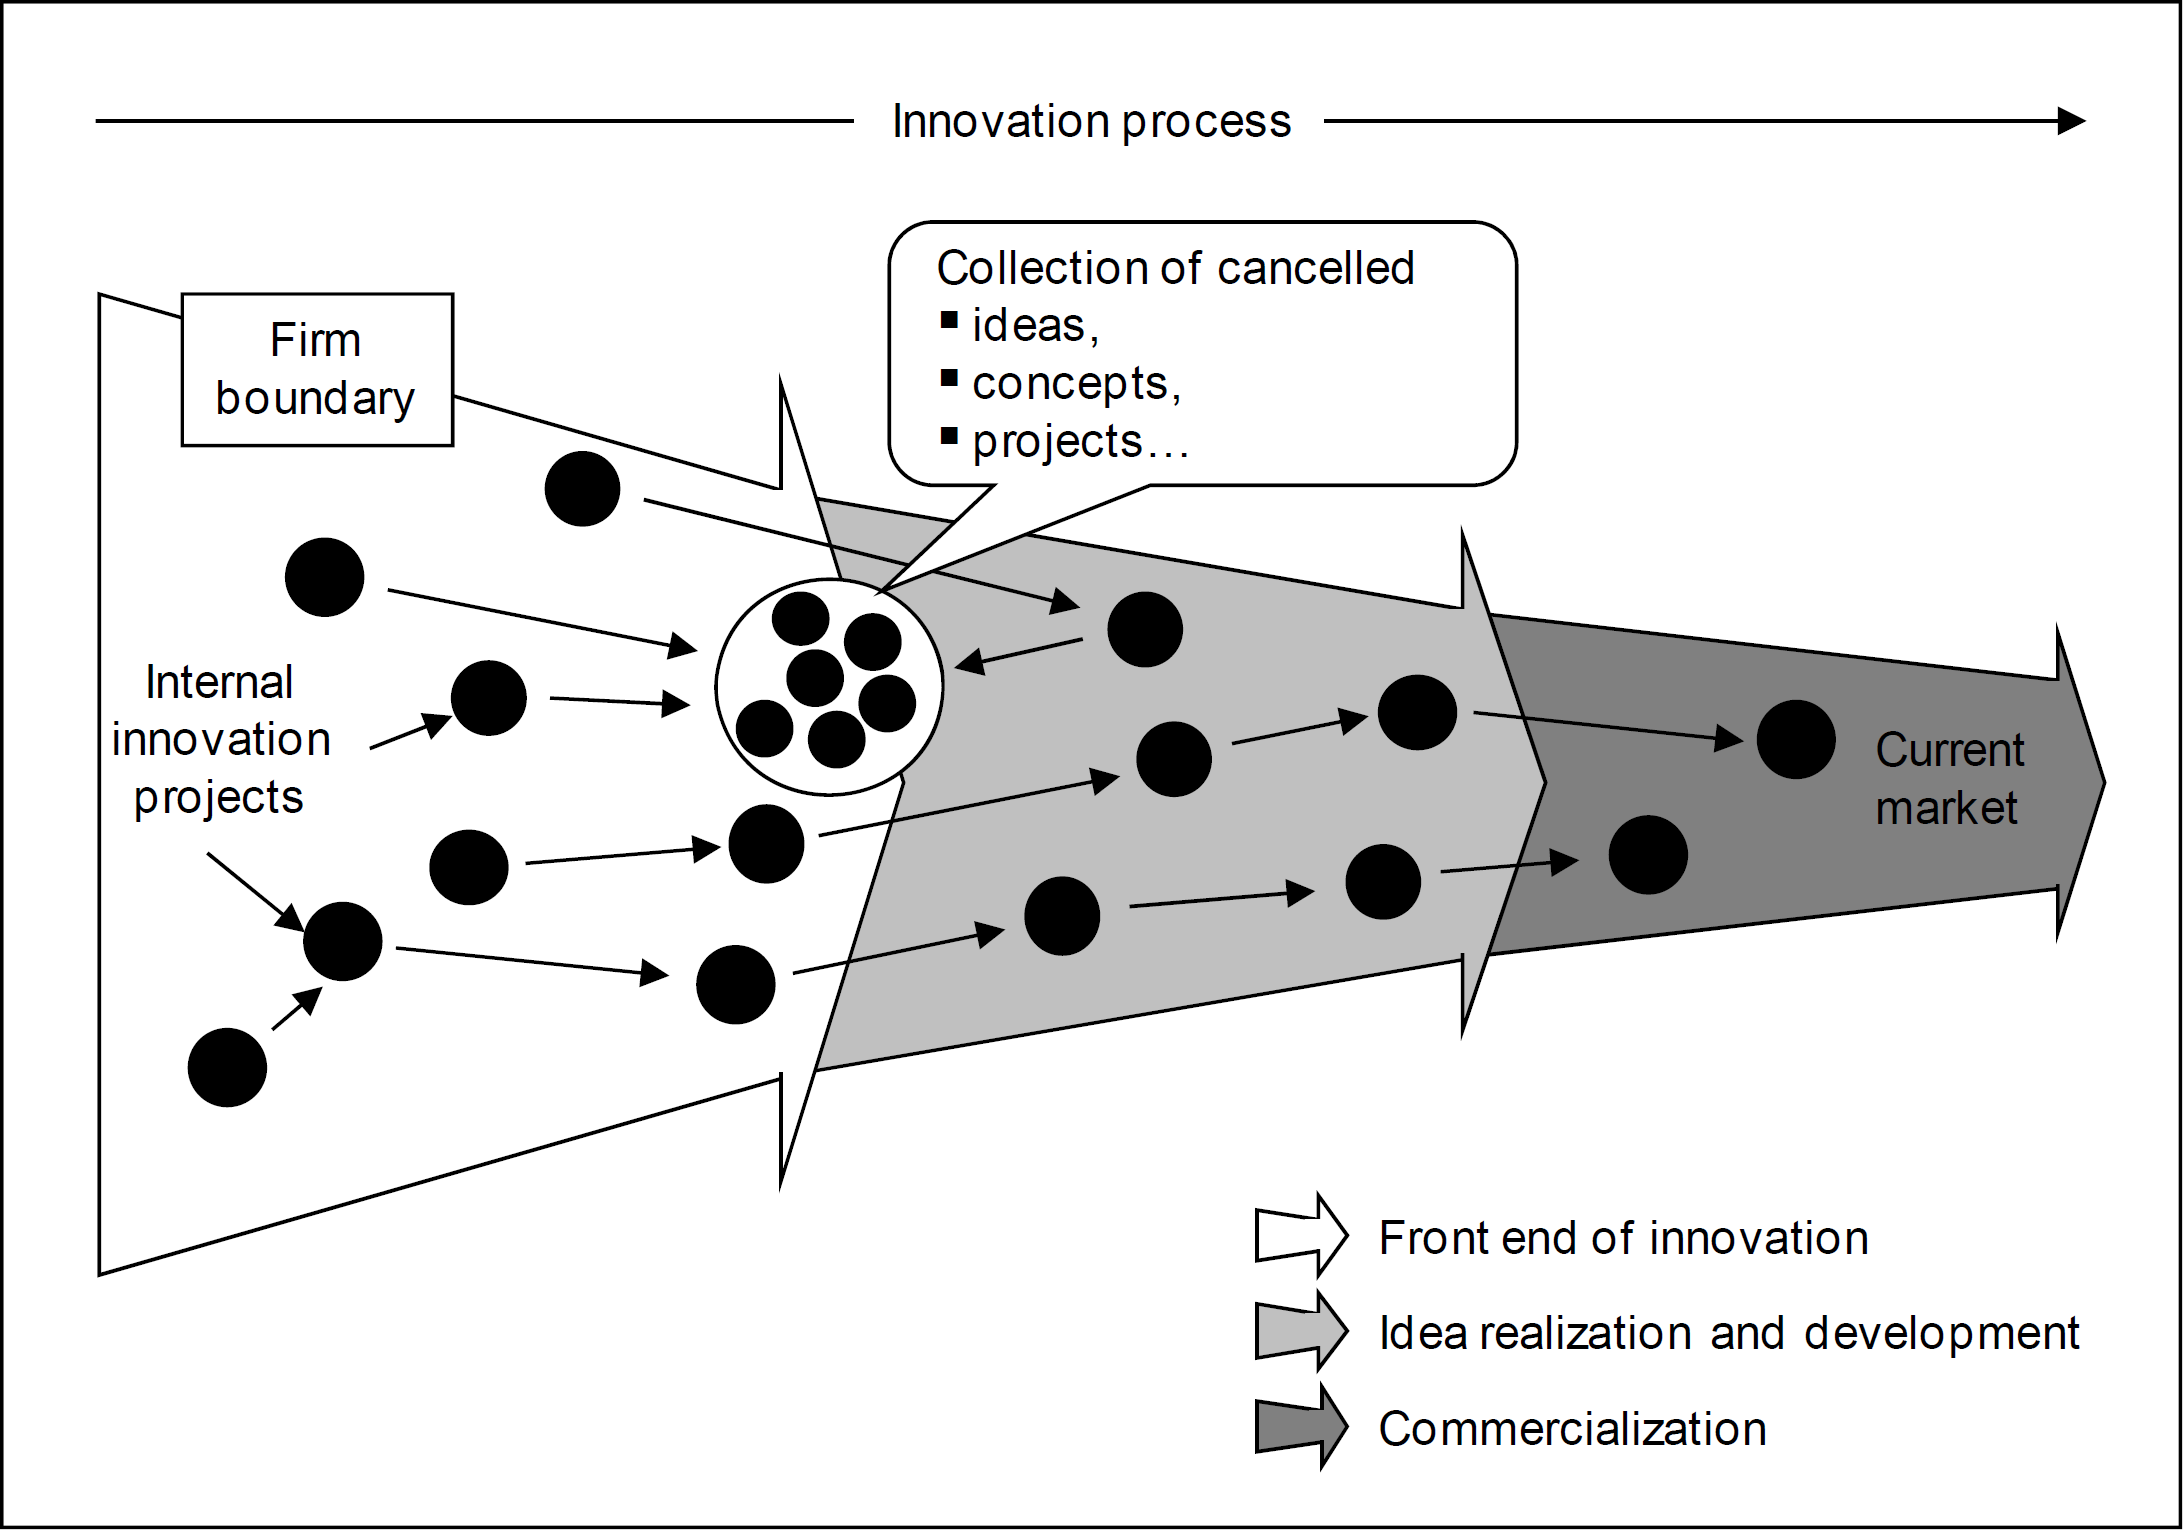
\includegraphics[width=1\textwidth]{ClosedInnovation}
    \caption{Closed Innovation Modell (aus \cite[20]{herzog2011})}
    \label{fig:closedInnovation}
\end{figure}

Selbstverständlich können nicht alle Ideen realisiert werden.
Möglicherweise ist die Ursache hierfür fehlende Ressourcen (Arbeitskraft oder Wissen)
oder es findet sich innerhalb der Unternehmensgrenzen keine vermarktbare Anwendung für eine neue Entdeckung.
Auch werden Ideen gegebenenfalls nicht umgesetzt, da vermutet wird, dass keine Akzeptanz am Markt herrscht.

Abgelehnte Ideen und abgebrochene Projekte werden beispielsweise in Datenbanken gesammelt.
Von dort werden sie wieder aufgegriffen oder bleiben ein ungenutzer Teil des geistigen Eigentums einer Unternehmens.


\subsection{Open Innovation}\label{sec:grundlagen-open}

Das Modell der \textit{Open Innovation} ist -- schon rein namentlich -- der Gegensatz der \textit{Closed Innovation}.
Da der Fokus dieser Arbeit auf letzerem liegt,
wird im Folgenden der offene Ansatz lediglich oberflächlich behandelt.
\todo[inline]{... um später besser Vergliechen zu können?}

\begin{figure}[ht!]
    \centering
    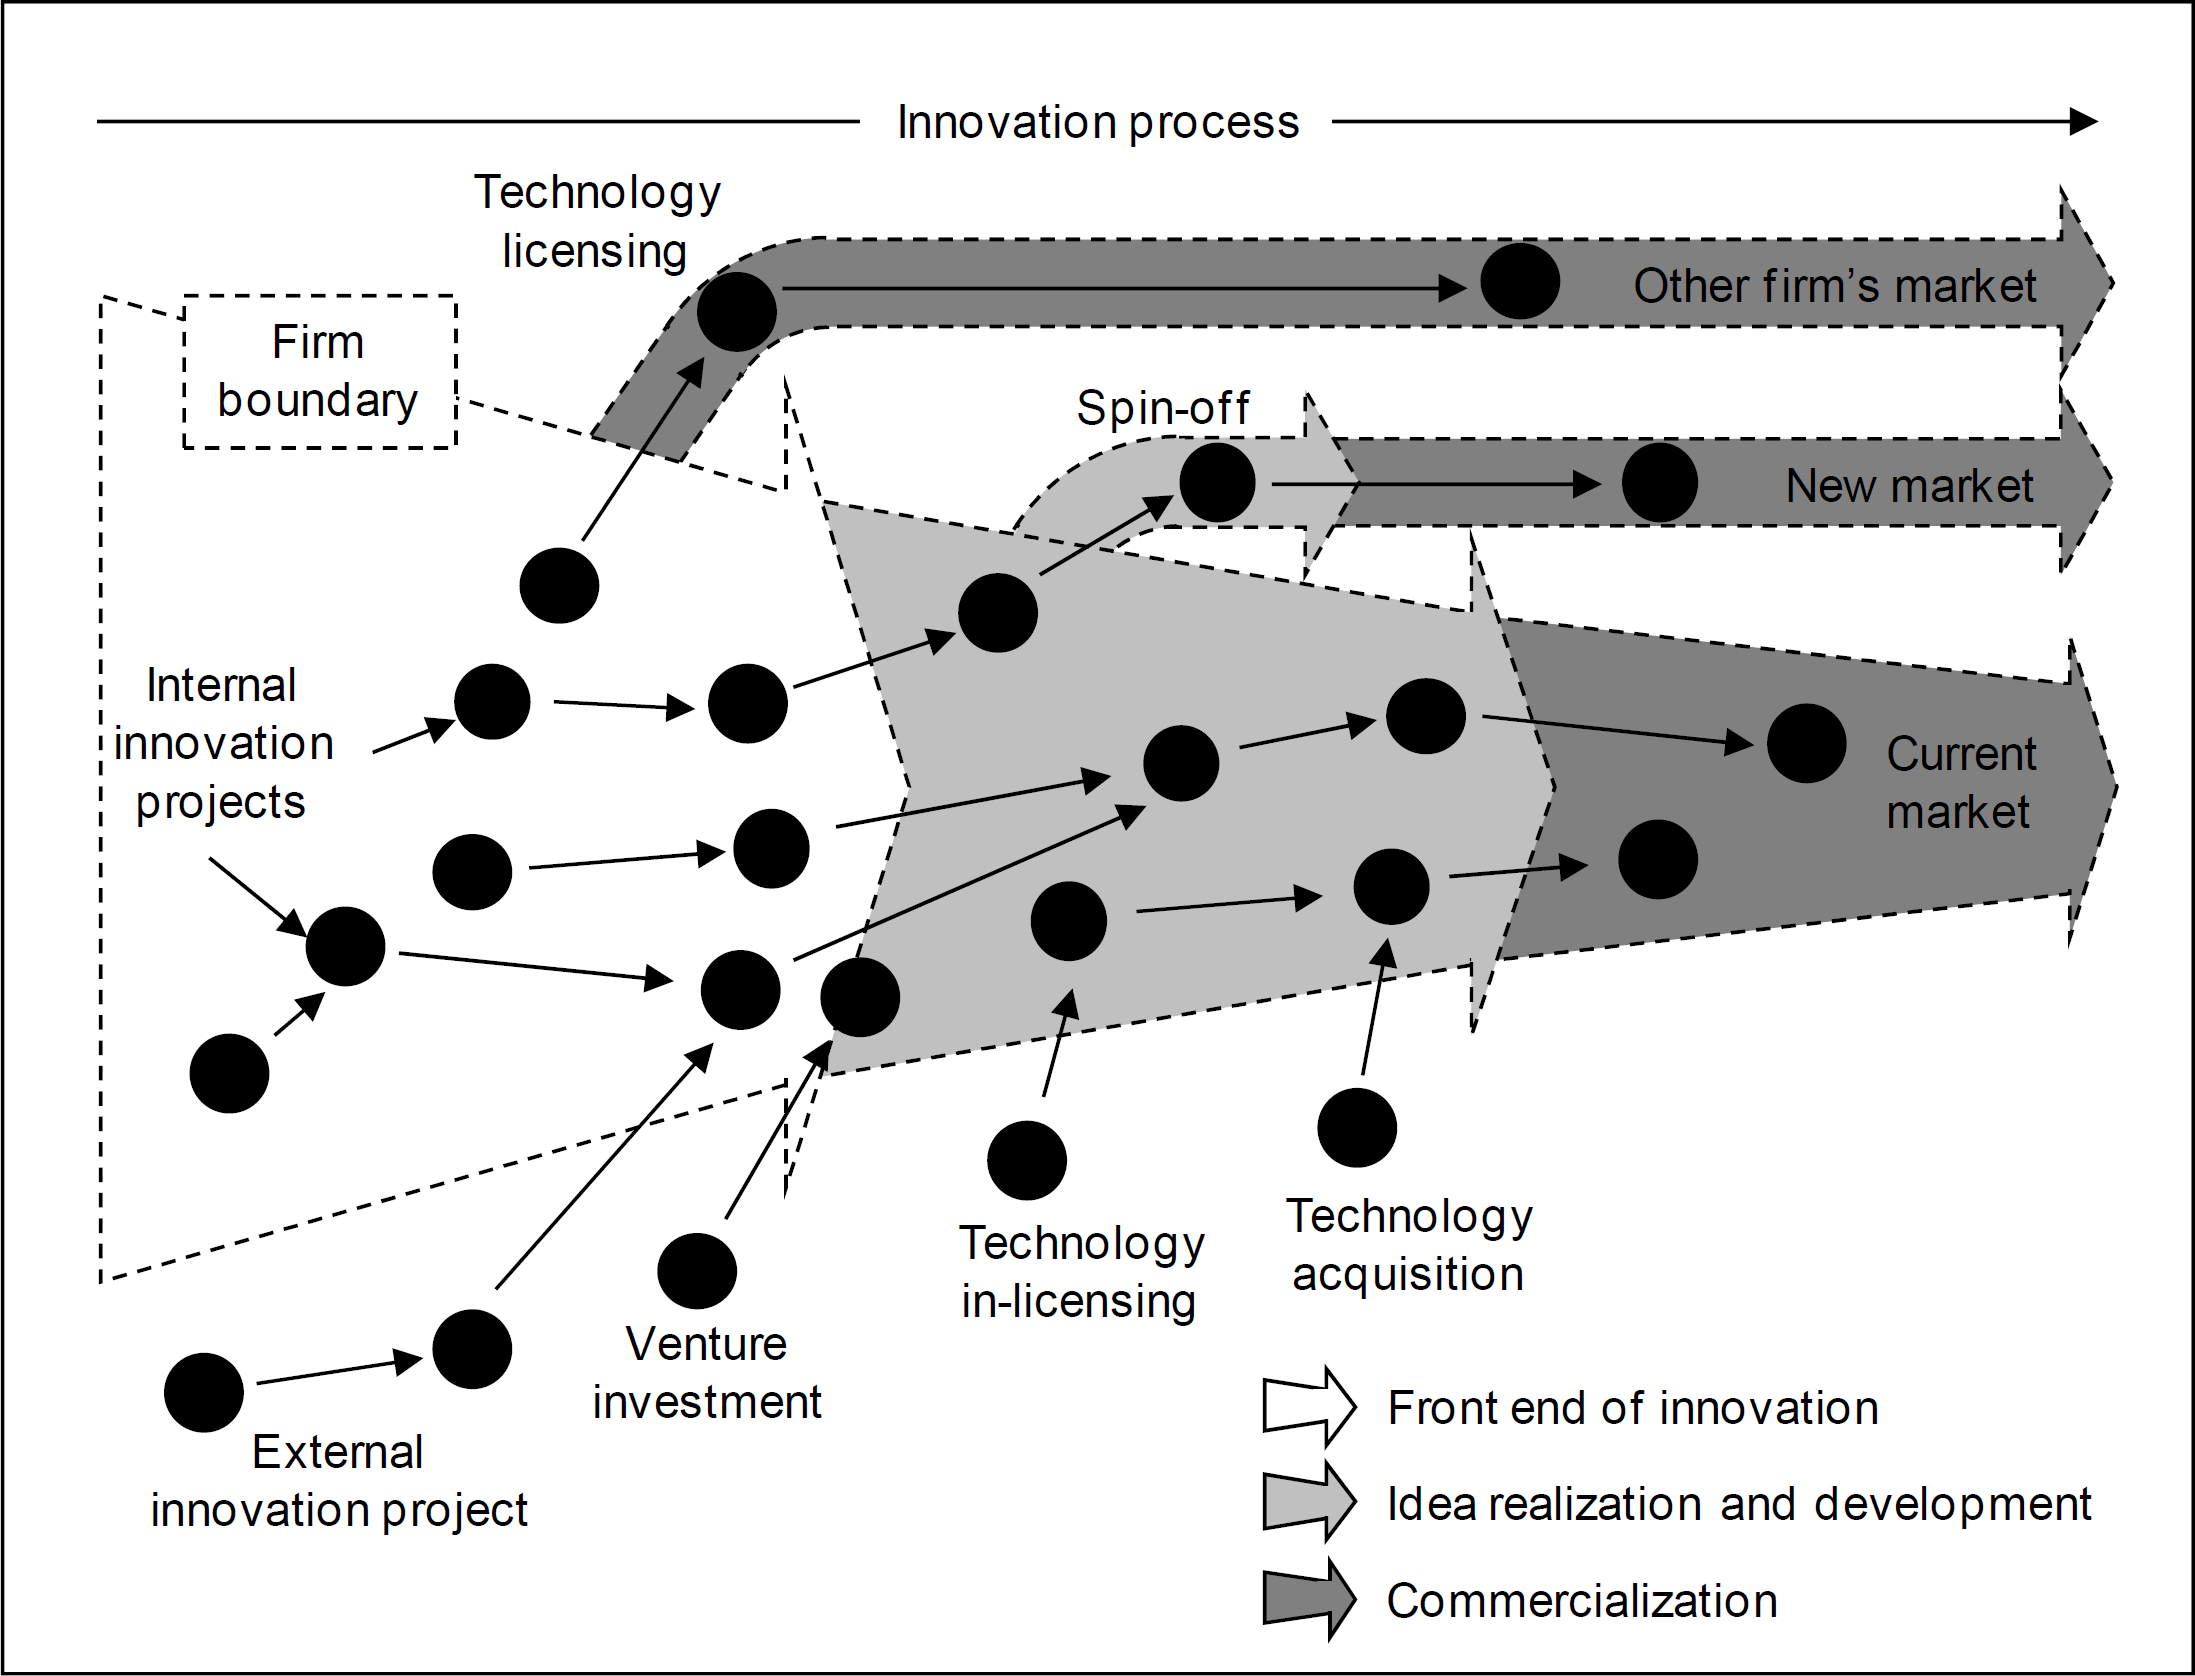
\includegraphics[width=1\textwidth]{OpenInnovation}
    \caption{Open Innovation Modell (aus \cite[23]{herzog2011})}
    \label{fig:openInnovation}
\end{figure}

Wie in \autoref{fig:openInnovation} zu sehen,
sind in der \textit{Open Innovation} die Grenzen eines Unternehmens \enquote{löchrig}.
Dies bedeutet, dass zusätzlich zu den intern entstandenen und entwickelten Innovationen
zusätzlich jederzeit Wissen von außen in den Innovationsprozess einfließt
und Projekte, welche innerhalb des Unternehmens nicht weiter verfolgt werden,
veröffentlicht werden oder genutz werden um neue Märkte zu erschließen.

Details zum \textit{Closed Innovation}-Ansatz können in unter Anderem
in \cite[60\psqq]{chesbrough2003} und \cite[21\psqq]{herzog2011} nachgelesen werden.